% !TEX root = thesis.tex

\section{Evaluating Social Signal Prediction}
\label{section:evaluation}
The output of social signal prediction should satisfy the following two requirements: (1) the predicted signals should be within a feasible human motion space showing realistic human motions, and (2) the predicted signals should follow the social rules, responding to the behaviors of communication partners. However, it is challenging to evaluate these requirements, because there is no objective metric to quantify ``realistic" or ``social" properties in behaviors. Notably, the L2 distance between the predicted signals and ground-truth may not be a good metric because it also does not consider such properties. For example, although several human behaviors can be still acceptable given the same input in our social signal prediction task, this metric penalizes them if they are different from the single ground-truth motion, regardless their quality. Due to the reason, the L2 metric often favors the output close to the mean of the data distribution, although it is qualitatively far from the expected output. The similar issue has been discussed in human motion forecasting field~\cite{mnih2012conditional, Fragkiadaki_2015_ICCV, jain2016structural, zhou2018autoconditioned}. In particular, we found that the first requirement can be satisfied by enforcing the output in the motion manifold space~\cite{holden2016deep}, but there is no good way to enforce the second requirement.


In this work, we present a way to quantify the quality of social signal prediction outputs (particularly body motion prediction), focusing on the turn-taking rule in social interaction (particularly for the second requirement). We found that the L2 distance is reliable for the signals in relatively lower dimensions, showing that the lower error clearly means the better quality. Classifying speaking status described in Section~\ref{subsection:ssp_pred_speak} is an example of it.  Our idea is to ``guess" the speaking status of the predicted body motion, and quantify it by using the ground-truth speaking status, as shown in Figure~\ref{fig:evaluation_bySpeakclass}. This method potentially penalizes only the turn-taking rule in the social situation, allowing diverse motion outputs as correct answers. To satisfy the turn-taking rule, the model still needs to learn the social rules by observing the input social signals. To produce speaking status from the predicted body gestures, we use our speaking status classifier described in Section~\ref{subsection:ssp_pred_speak}. This metric is not ideal due to the use of our speaking status classifier which is not perfect, and also due to the fact that it only penalizes a subpart among many social rules. However, we found that this metric provides a more reliable way to quantify body motions than L2 distance. 


%Good metric is also closely related in training a better model, because the metric can be directly used as a loss function in learning stage. for loss function in the neural network architecture. This is one of the biggest challenging in evaluating the performance of the social signal prediction, and it also related to the loss function in training our models.





%penalize the realist signals if it is deviated from the ground-truth. As an example, in our in synthesizing body gestures, a mean of the entire pose distribution shows very competitive L2 errors compared to predicted output, although qualitatively the mean pose does not satisfy either requirements. Similar issues have been discuss in the forecasting single person's human motions~\cite{mnih2012conditional, Fragkiadaki_2015_ICCV, jain2016structural}. It should be noted that the same metric is also used in training models (e.g., neural network), which makes the output of the model converges to the mean pose in the end. 




%The work in forecasting motion of a single subject focuses on the first requirement~\cite{mnih2012conditional, Fragkiadaki_2015_ICCV, jain2016structural}, and the area suffers from the deficiency of a good evaluation method. The L2 distance between the predicted signals and ground-truth motion is often used


% while the second requirement is more challenging and rarely demonstrated. For example, any arbitrary ground-truth motion capture data can satisfy the first condition (because they are genuine signals of humans), and arbitrary combinations of such motions with smooth transition still can satisfy the condition~\cite{kovar2008motion}, but the second condition can be achieved by properly modeling social communication.
%
%Both requirements are hard to be evaluated.
%
%Good metric is also closely related to learining better model, because the metric can be directly used for loss function in the neural network architecture. This is one of the biggest challenging in evaluating the performance of the social signal prediction, and it also related to the loss function in training our models.
%
%
%We found for some subpart of signals, this L2 metric provided consistent output as in qualitative evaluation, for example, in speaking classification and social formation estimation. They are hard to be applied for more high dimensional signal such as body signal. 
%
%
%
%We can use a human manifold space to evalute the first requirement. If output is far from this manifold space, then we can consider they are less realistic motion; that is the distance between the projected point to the original signal would be an evaluation metric. However, this requires a well-defined manifold space, which is a challenging issue. Moreover, since our motion output are synthesized by this manifold model, they tend to located in the space already, providing biases in evaluation. This output is discussed in Section~\ref{chapter:manifold_metric}. 
%
%The second requirement is very challenging without objective way to measure, due to the inherent diversity of human behaviors. Given an input signals of others, there could be several possible reaction of humans, which all can be possible solution, if it is within our social norms. A common evaluation metric, L2 distance, may penalize the realistic motion if it is far from the ground truth motion measured in our system. 
%
%We present an indirect method as a way to quantitatively measure the quality of prediction output. We use our trained network which takes body motions and produces signals which can be more reliably evaluated (e.g., speaking signals). Since the timing of speaking is closely related to the social interaction (turn taking), it can be used to evaluate the social requirement. We found that this method shows a reasonable output by penalizing the mean pose and favor the qualitatively better estimation output. This output is discussed in Section~\ref{chapter:classifier_metric}. 



\begin{figure}
	\centering       
	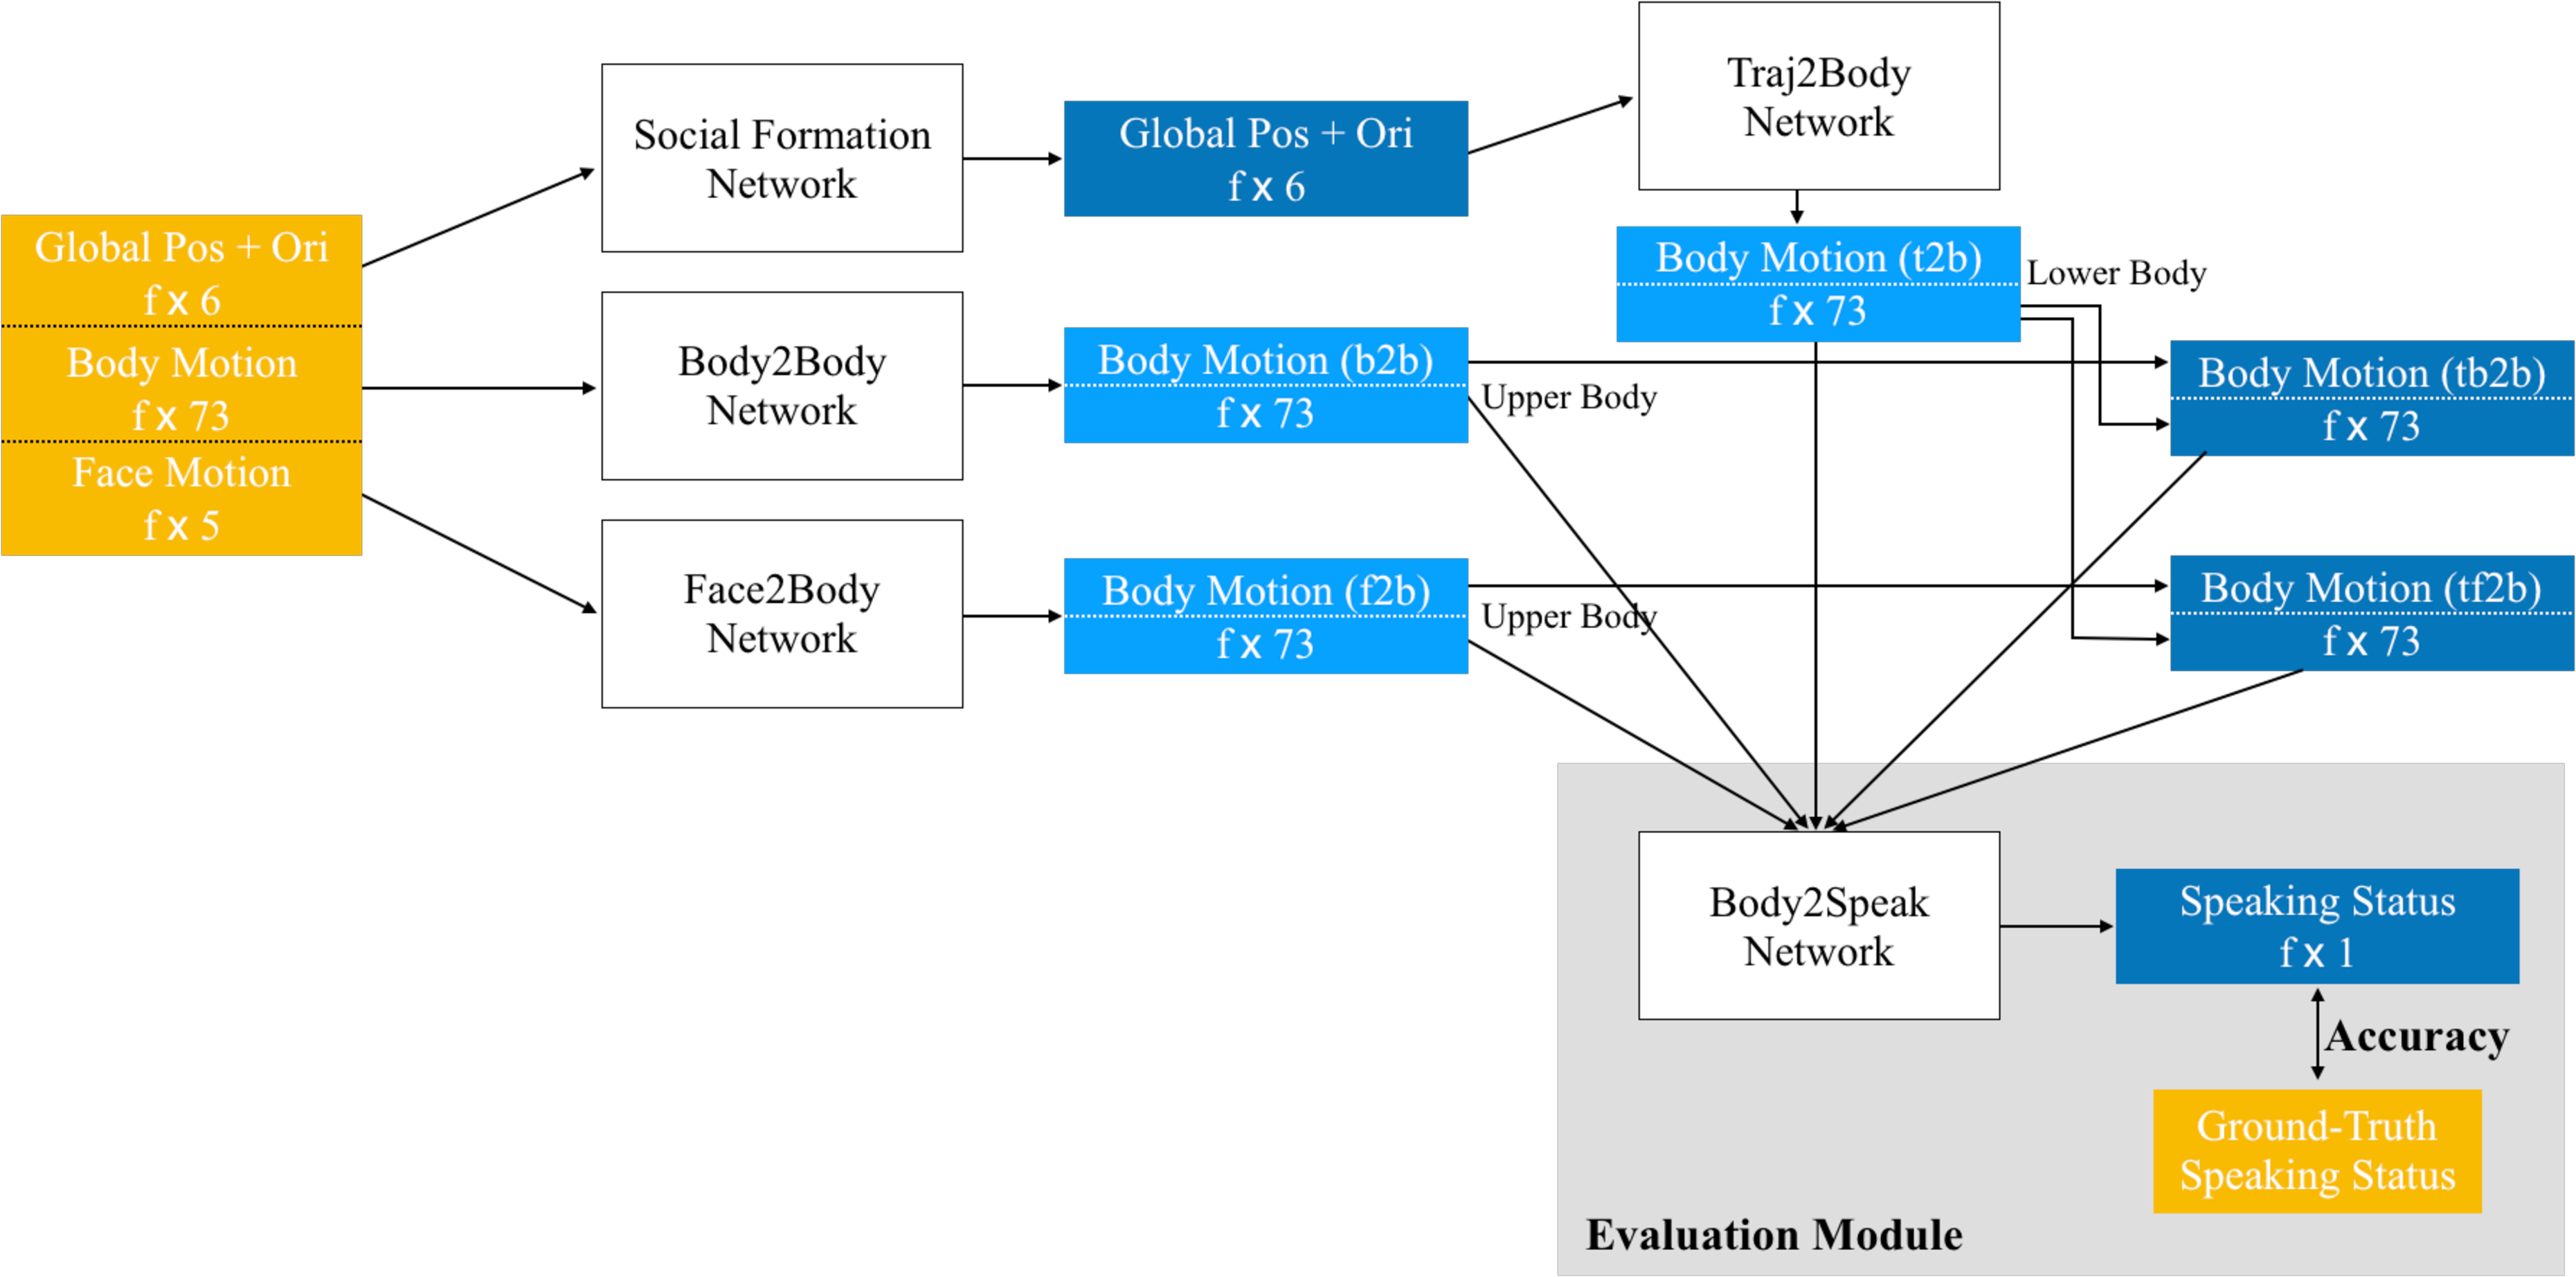
\includegraphics[ width=0.8\linewidth]{ssp_fig/evaluation_pipeline.pdf}
	\caption{Evaluating body motion prediction by speaking classification} 
	\label{fig:evaluation_bySpeakclass}
\end{figure}


\section{Results}
In this section, we show experimental results in predicting the several important social signals from different input sources. The core direction in performing this experiments is to explore the correlations of diverse behavioral channels measured in genuine social communications. We leverage the wide spectrum social signal measurements of the Haggling dataset, and train neural network models to predict the social signals of the target person, including speaking status, social formations (positions and orientations), and body gestures.

\subsection{Pre-processing Haggling Data}
Given the motion data of the Haggling games, we first annotate the start and end time of the game, where the start time is decided when the social formation is built and the end time is defined when the social formation is broken. We crop out the motion dataset based on this start and end time, so that we ignore the time while subjects enter and exit the capture space. For each haggling game scene we also annotate the roles in the game, buyer, left-seller, and right-seller, where the left and right are determined in the buyer's viewpoint. In our experiment, we specify that the left seller is our target person and predict the social behavior of these subjects. Following the work of~\cite{holden2016deep}, we re-target the motion data to a standardized skeleton size to remove size variation from the body skeletons. We also synthesize footstep signals and decouple the body motion from global translation and orientation using the method of ~\cite{holden2016deep}. Finally, we divide the dataset into 140 training sets and 40 test sets. However, since there exist sequences where the reconstruction errors are severe for some frames, we select only 79 training sets and 28 testing sets which are manually verified to be error free. Although our dataset captures face and body signals, we do not include these data in our current experiments. 


\subsection{Verification of Proxemics}
An interesting experiment is to consider the well-know theories in psychology again using the new data we collected in our sensor system. Our dataset has the measurement of fully spontaneous motions (including the position and orientation of groups) of interacting people, and enables us to revisit the well-known proxemics theory~\cite{Hall66}. We first compute the average distance between a pair of subjects: (1) buyer and right sellers (B-RS), (2) buyer and left seller (B-LS), and (3) left seller and right seller (LS-RS). The results are shown in Table~\ref{table:proxemics_comp}. We found that the result approximately follows the social distance categories defined in the Hall's categorization~\cite{Hall66}. The distances among sellers are within the close phase of social distance ranges (from 120-210 $cm$) and the average distance among sellers and buyers are within the far phase of social distance (from 210 to 370 $cm$) in \cite{Hall66}. To analyze the shape of the social formation, we plot the average formation of games in a person-centric coordinate by a buyer. The results are shown in the Figure~\ref{fig:socialgeo_distribution}, showing that the formation is often similar to isosceles triangles with relatively far distances between a buyer and two sellers than the distance between sellers. 


\begin{table}[t]
	\centering
%	\footnotesize
	\caption{Average distances (cm) between subjects. B, RS, and LS denote buyer, right seller, and left seller respectively.}
	\label{table:proxemics_comp}
	\begin{tabular}{c| c| c| c| c}
		\hline
		%Types & Avg. dist. (cm) & Std.(cm) & Min dist. (cm)  & Max dist. (cm)\\
		& Avg. dist. & Std. & Min & Max \\
		\hline
		B-RS & 148.11 & 27.26 & 99.03 & 265.52 \\
		\hline
		B-LS & 151.45 & 29.62 & 104.24  & 284.85 \\
		\hline
		LS-RS & 124.13 & 24.05  & 77.70  & 206.26 \\
		\hline
	\end{tabular}
\end{table}

\begin{figure}
	\centering       
	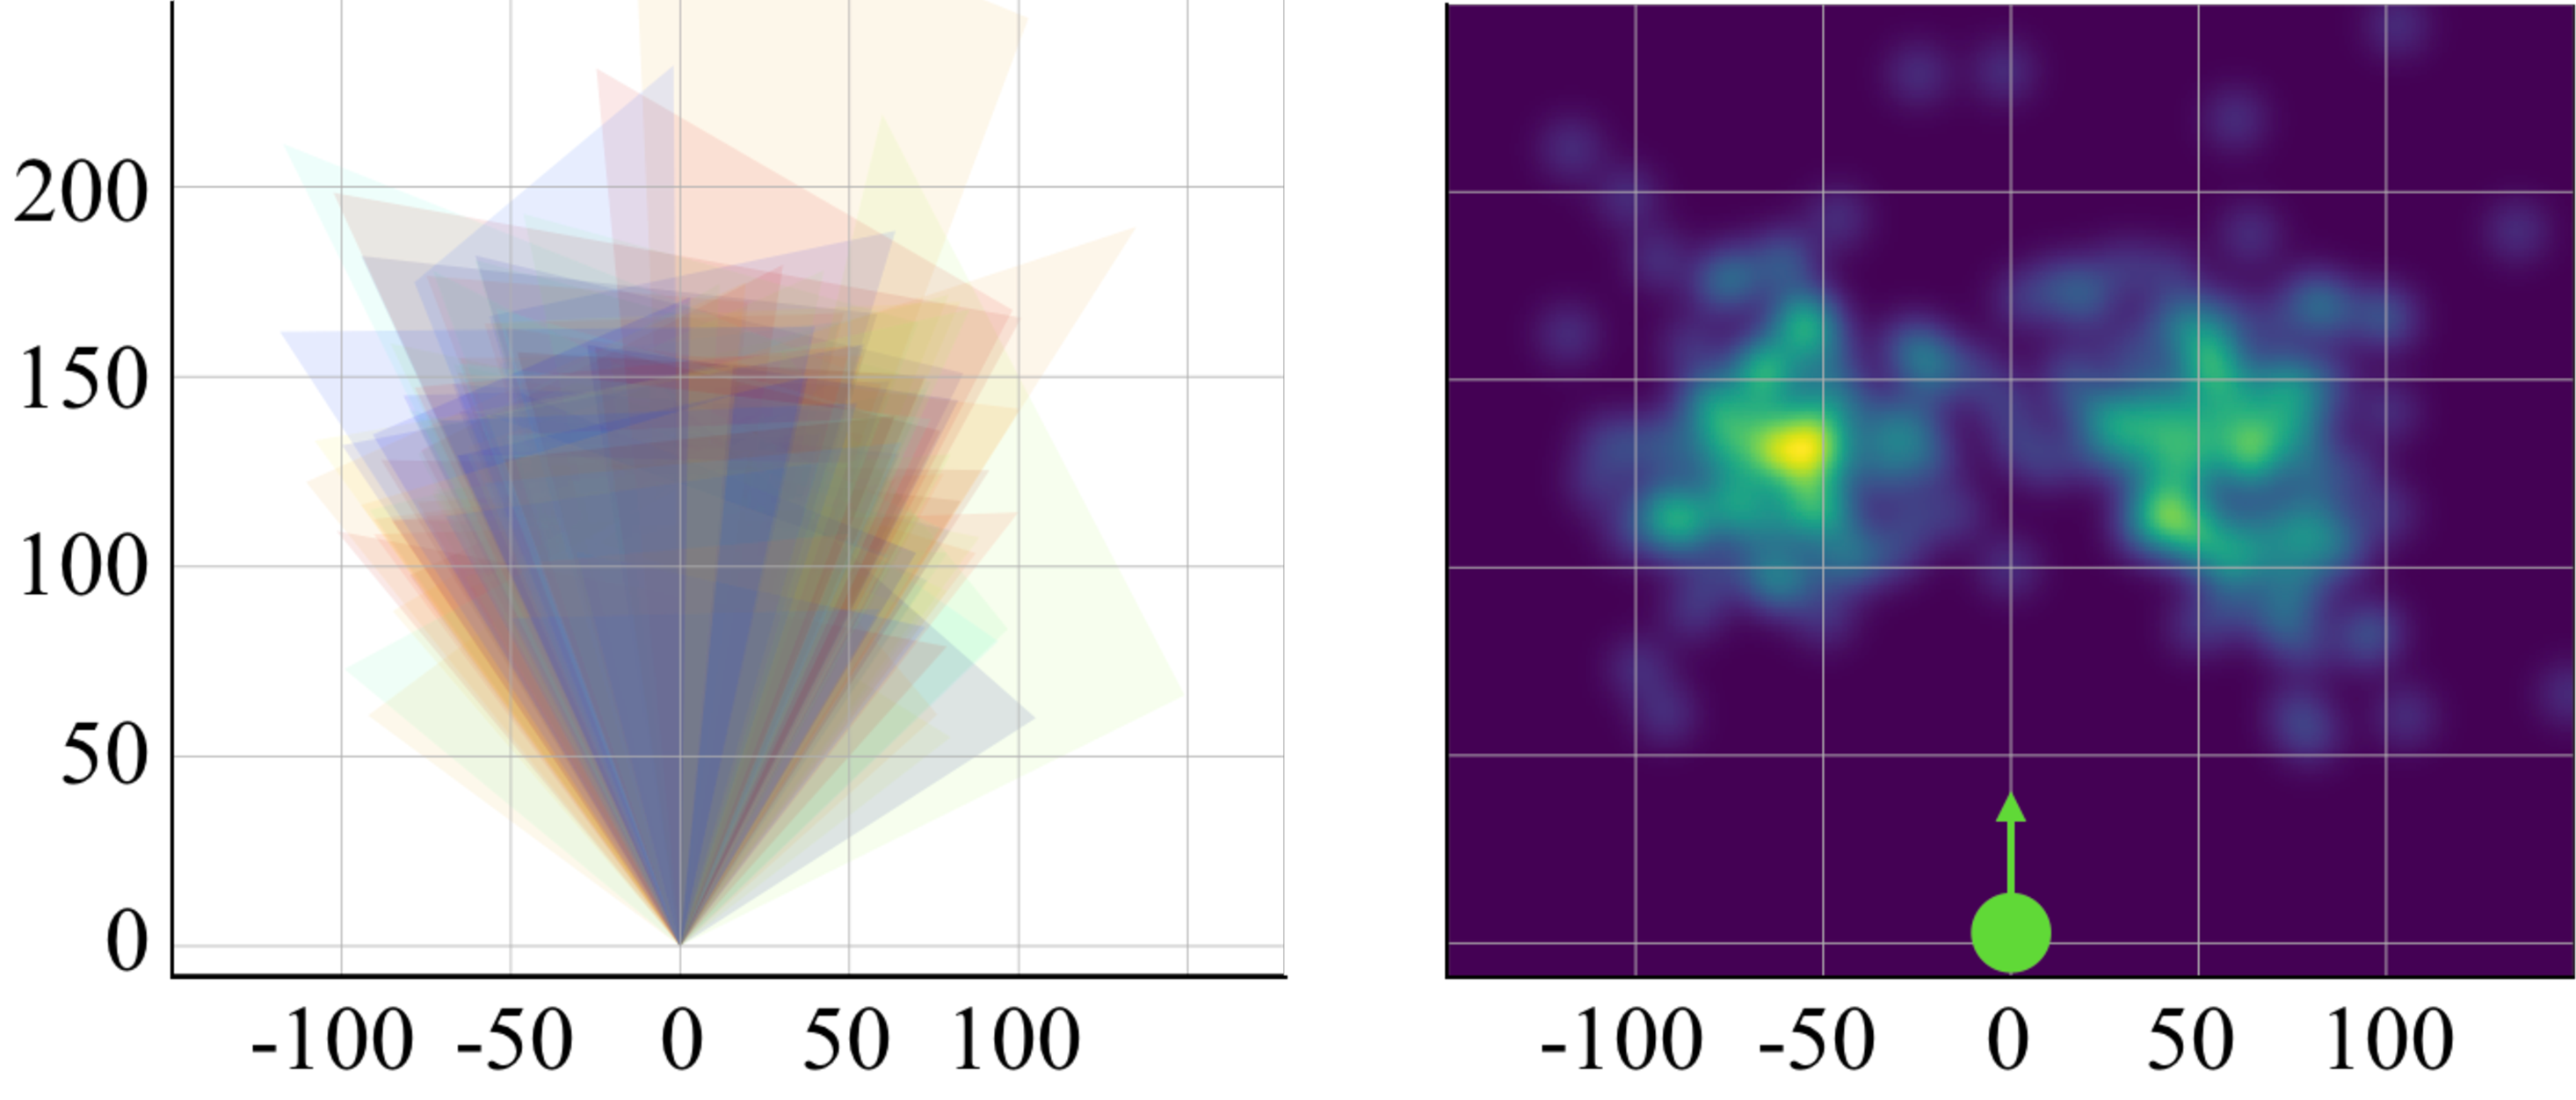
\includegraphics[ width=0.8\linewidth]{ssp_fig/haggling_proxemics_stat.pdf}
	% 	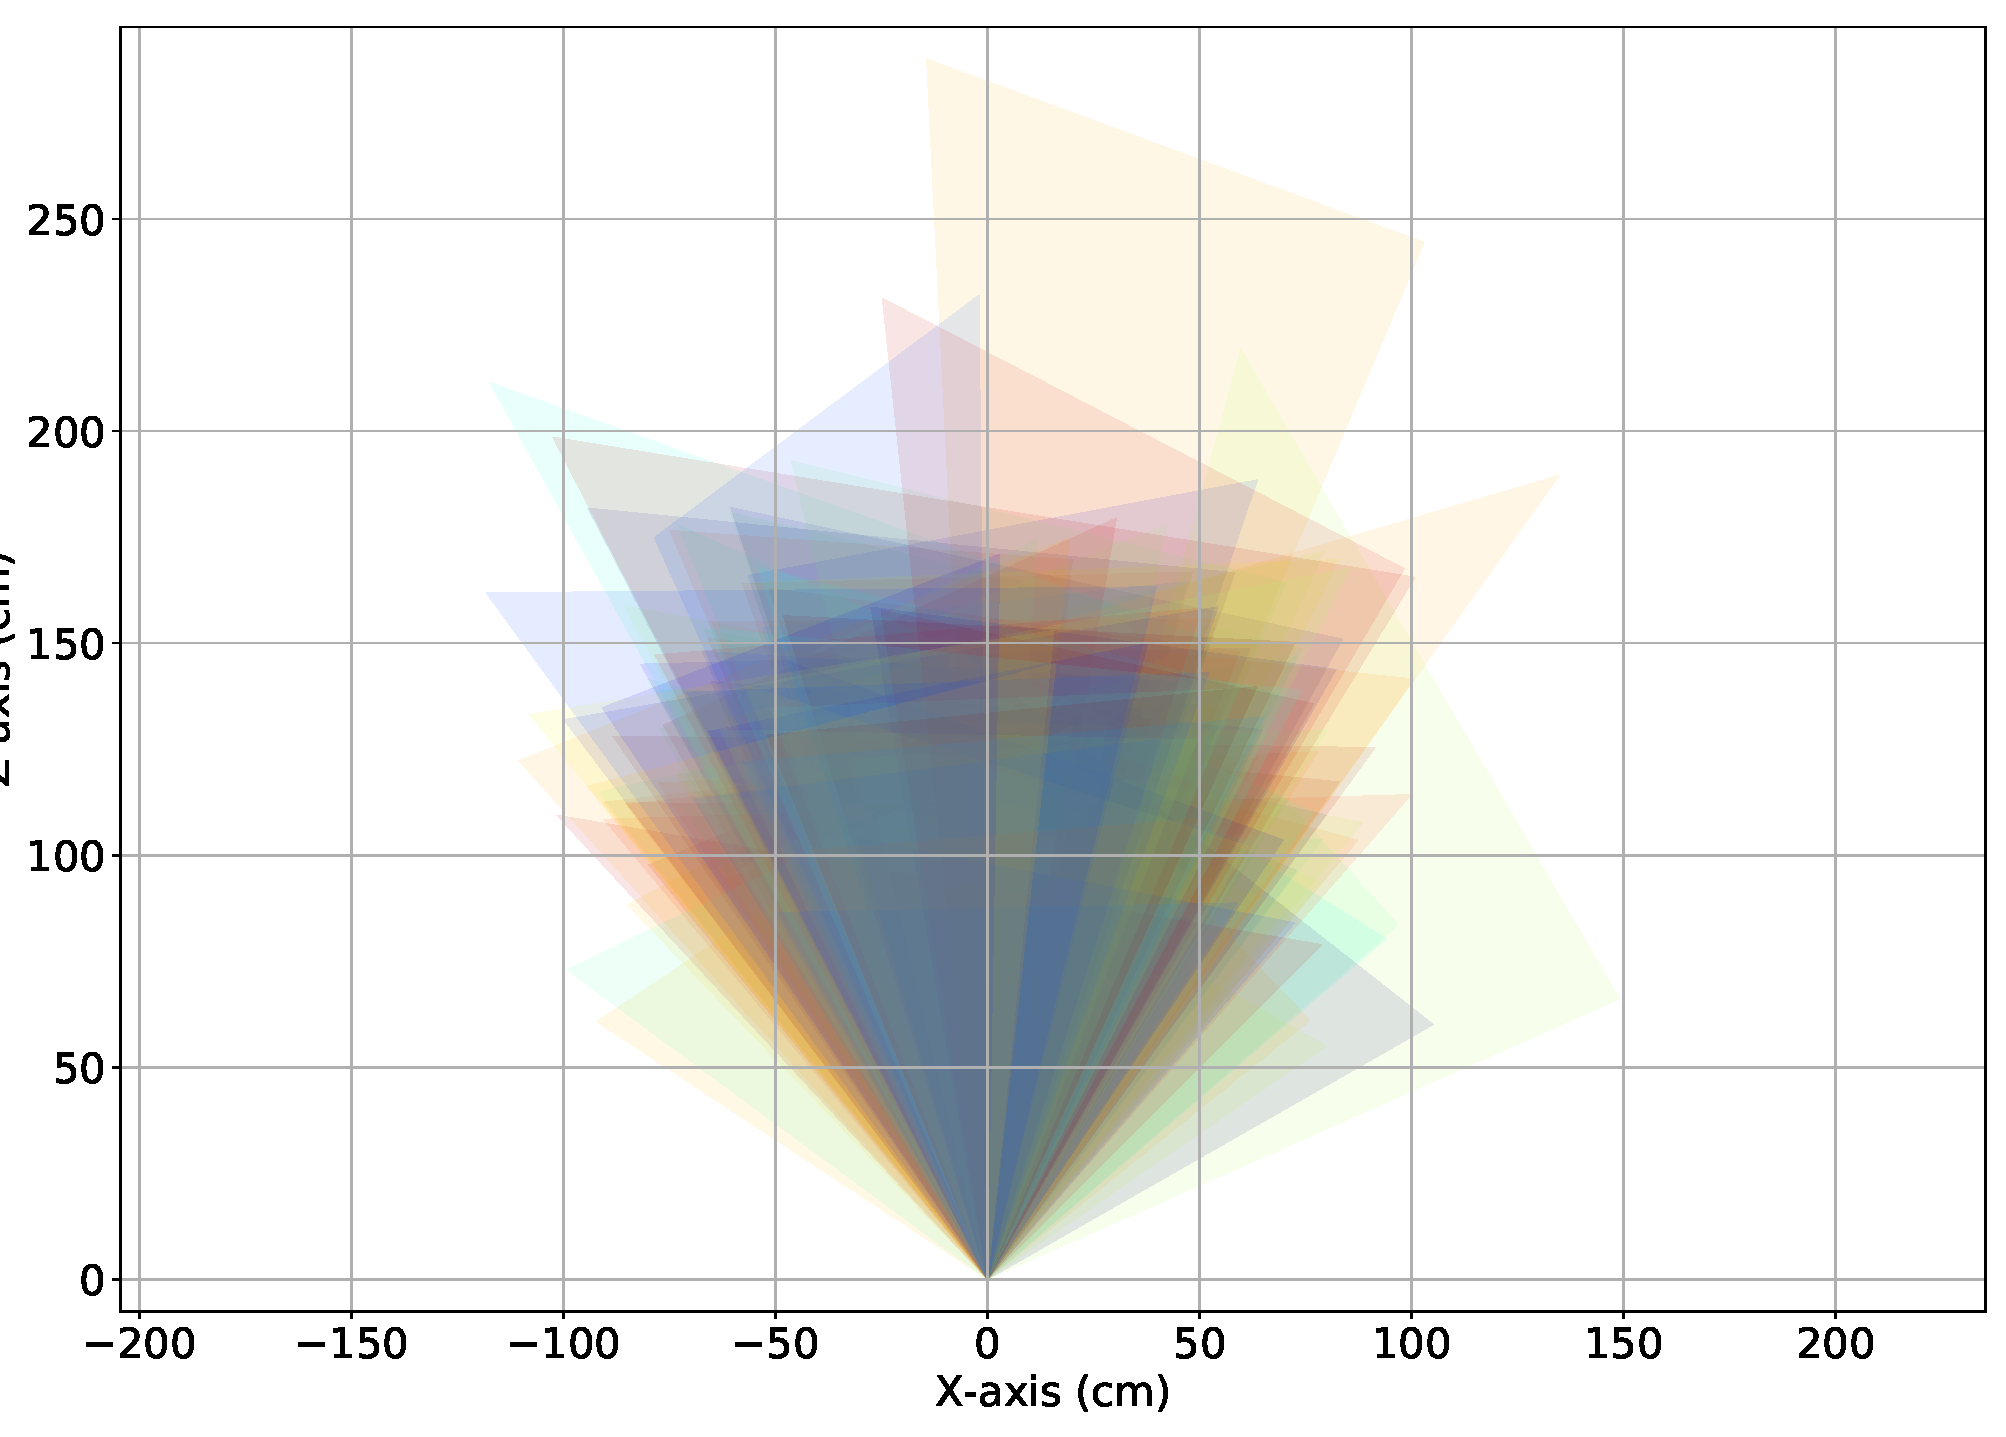
\includegraphics[trim=120 0 120 0,clip, width=0.45\linewidth]{plot/haggling_proxemics_polygon.pdf}
	% 	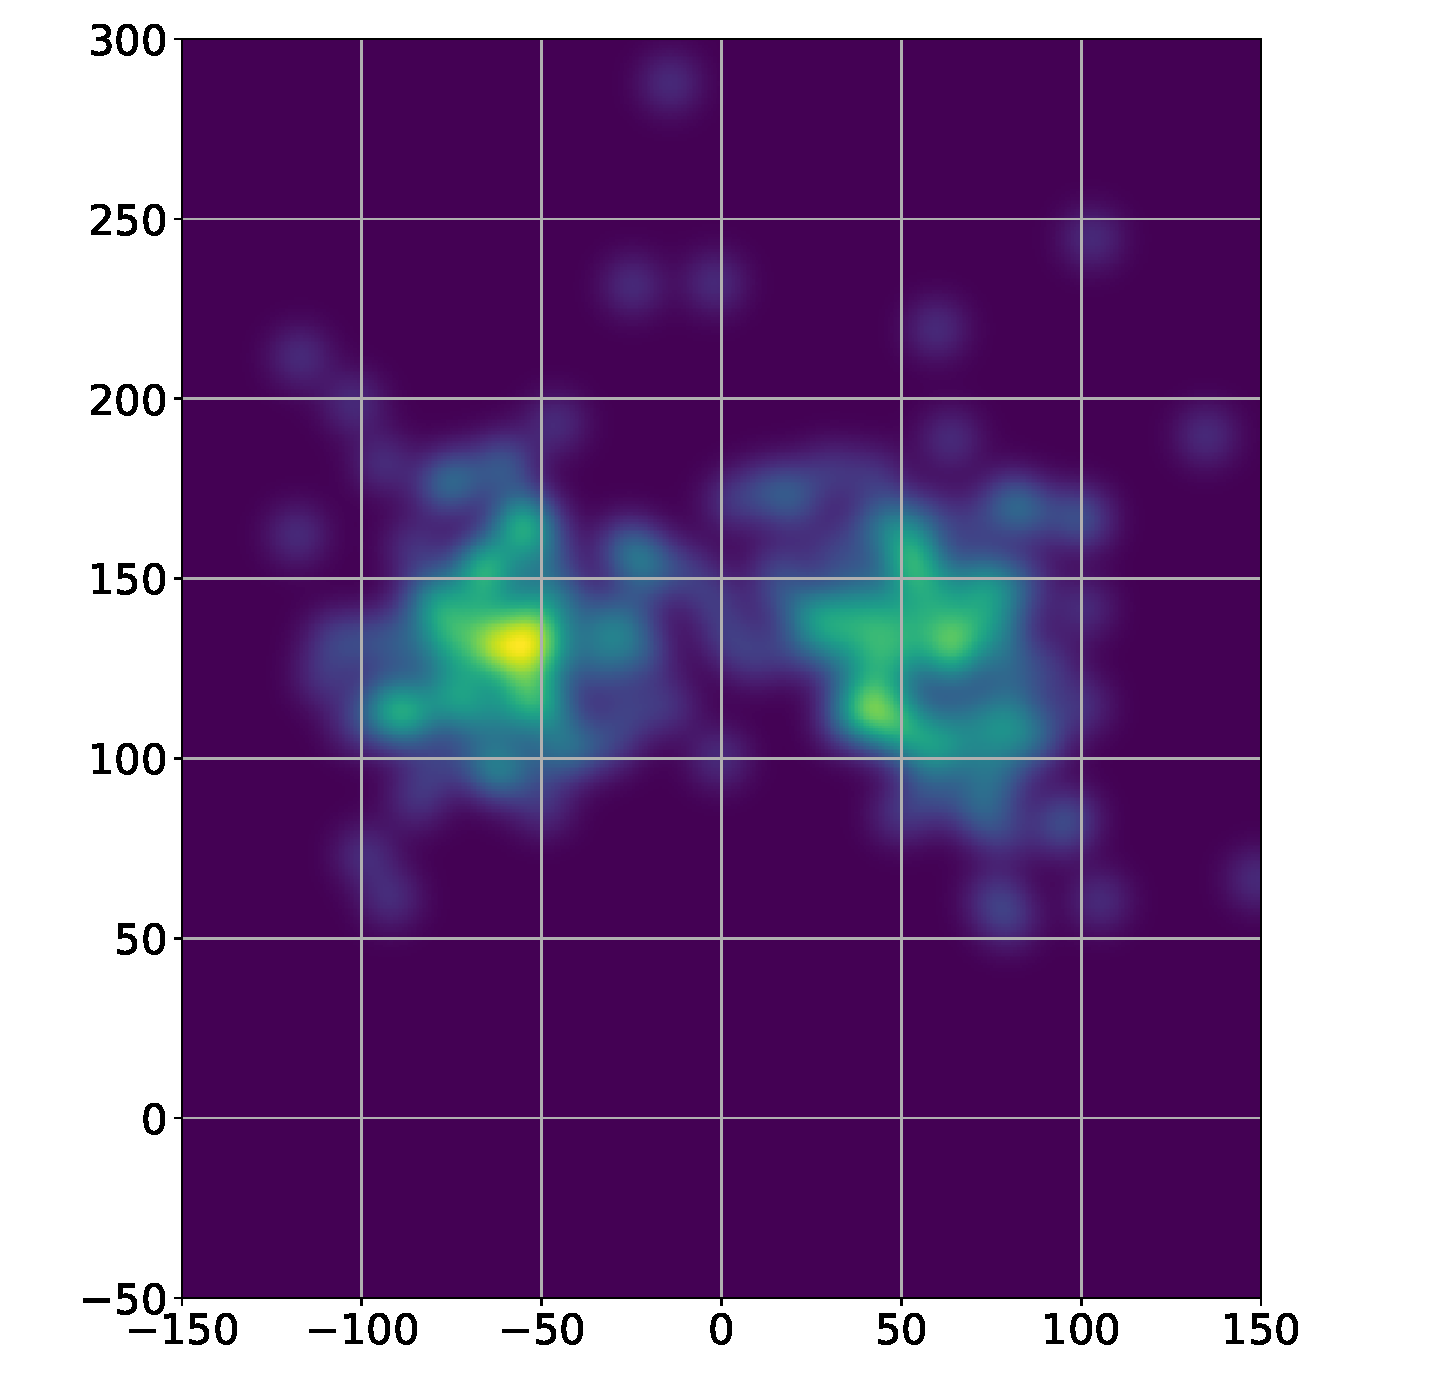
\includegraphics[width=0.45\linewidth]{plot/haggling_proxemics_heatmap.pdf} 
	%	\subfigure[TrajCompares]{\label{Fig:asso_traj}\includegraphics[width=0.5\textwidth]{img/trajCompare}}   
	\caption{Visualizing social formations in the haggling sequences as triangles (left) and a heat map (right). The formation is normalized w.r.t the buyer's location, and the green circle on the right shows the buyer location (origin) and orientation ($z$-axis).} 
	\label{fig:socialgeo_distribution}
\end{figure}

% \begin{figure}
% 	\centering       
% 	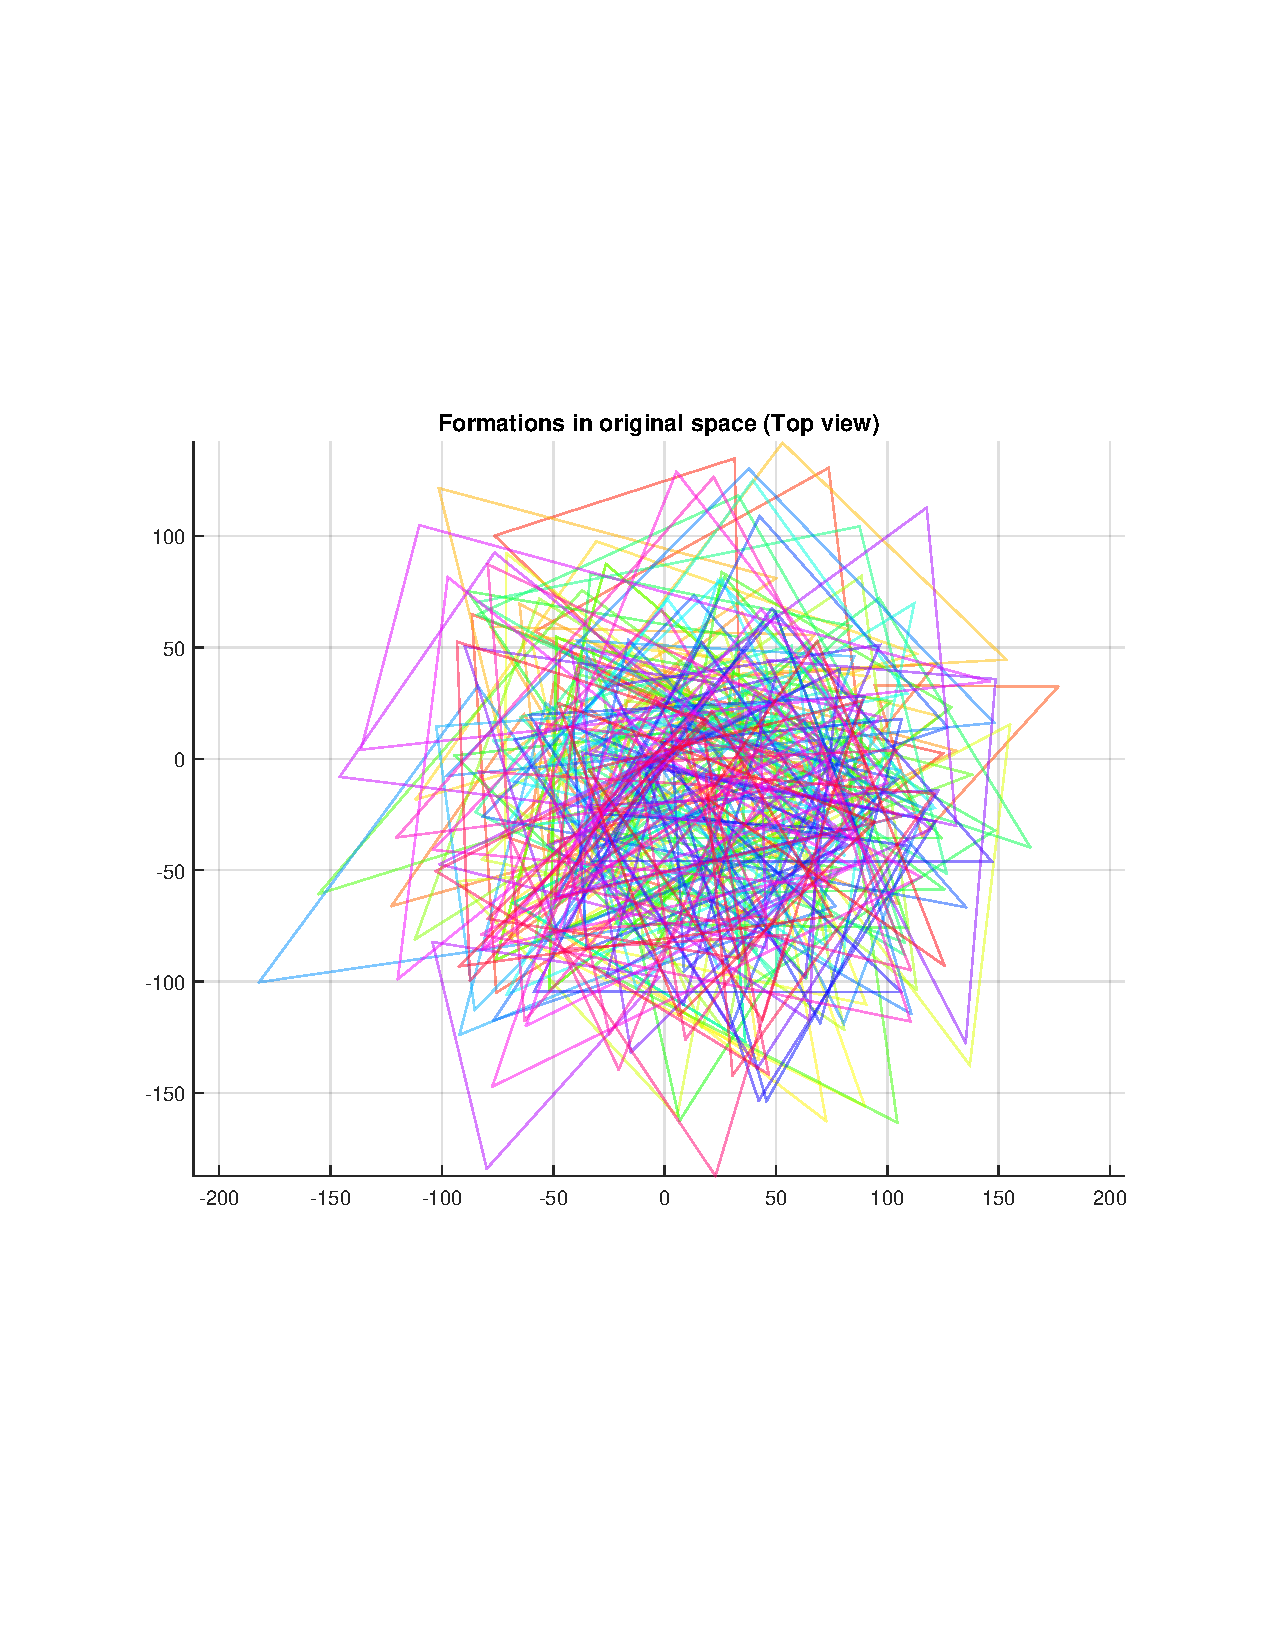
\includegraphics[trim=60 200 60 150,clip,width=0.32\linewidth]{fig/originalTri}
% 	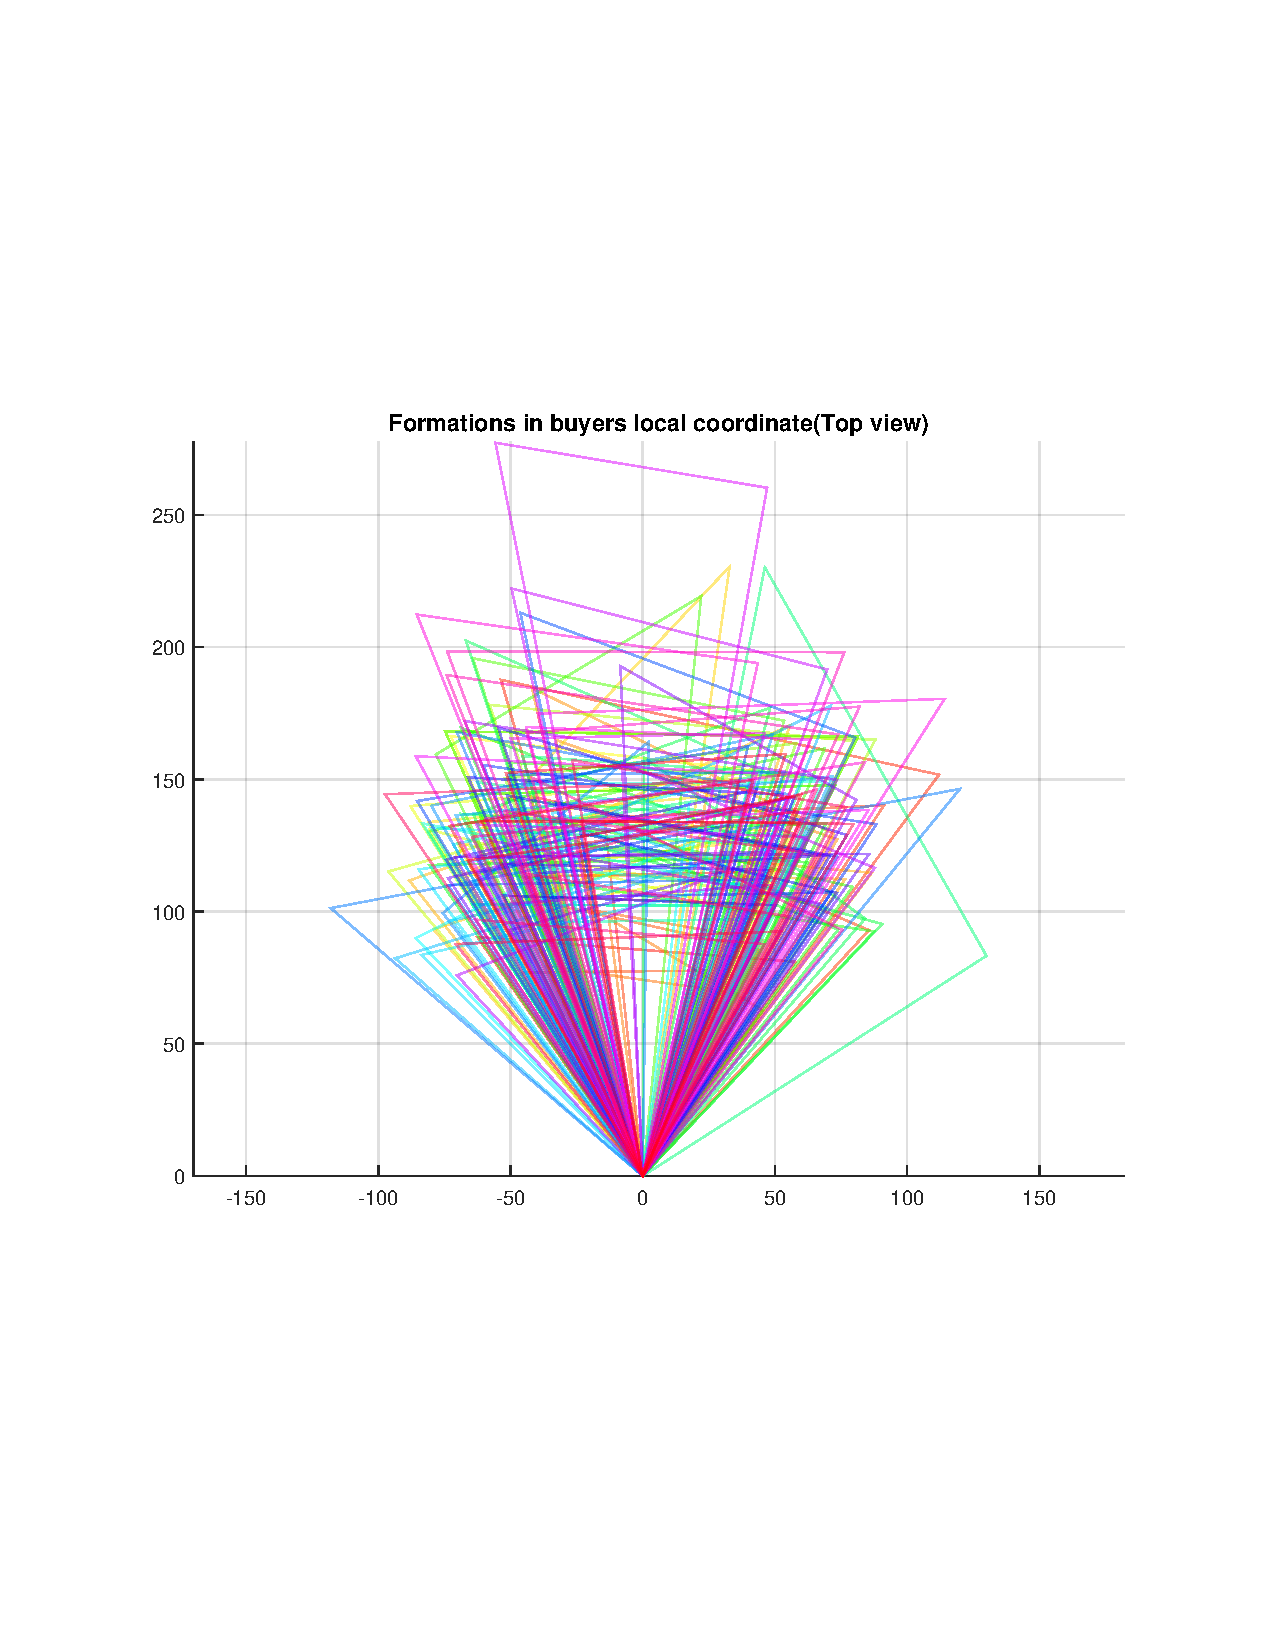
\includegraphics[trim=60 200 60 150,clip,width=0.32\linewidth]{fig/buyersTri} 
% 	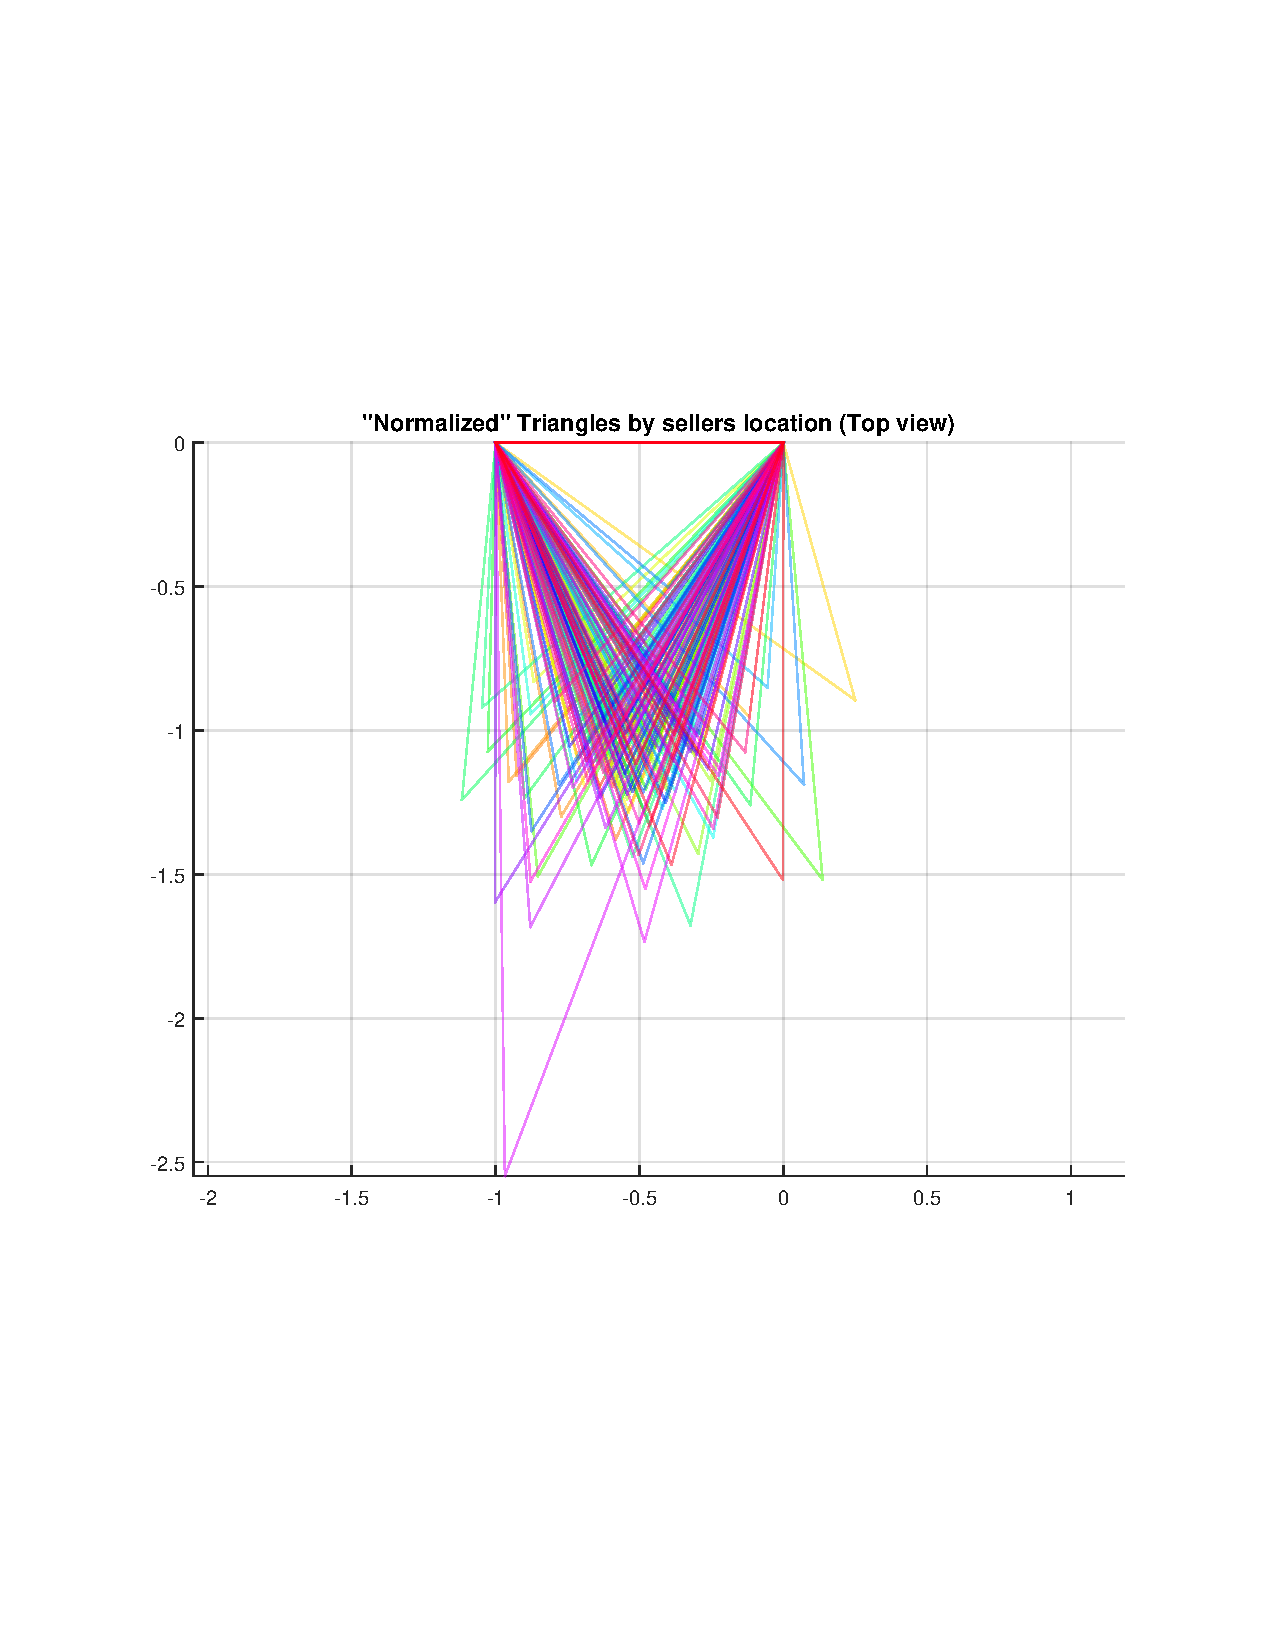
\includegraphics[trim=60 200 60 150,clip,width=0.32\linewidth]{fig/normTri} 
% 	%	\subfigure[TrajCompares]{\label{Fig:asso_traj}\includegraphics[width=0.5\textwidth]{img/trajCompare}}   
% 	\caption{Social formations in three different representations. (a) Global coordinate; (2) Person-centric coordinate defined by buyers; (3) Normalized-by-a-pair coordinate system define by two sellers} 
% 	\label{fig:socialgeo_distribution}
% \end{figure}

\subsection{Speaking Status Prediction}
We predict whether the target person is currently speaking or not by observing other social signals in the scene. First, we investigate the performance when the target individual's own social signals are used as input. Three different input sources--facial expressions, body gestures, and both of them---are used to train neural network models respectively. In particular, we use the same neural network architecture for this experiment by keeping the input dimension and network size to make the comparison as fair as possible. More specifically, we use the``body2speak" model in \ref{section:body2speak}, by modifying the input dimension into the concatenation of face and body signals (with $5+73$ dimensions). To test with only the body signals as input, we mask out the face signal part in the input with their average values. Similarly, we mask out the body part in the input to test with the face signal only.  The prediction accuracies from these input signals are shown in the first column of Table ~\ref{table:speaking_class}. In our result, the facial cue of the target person shows the strongest correlation (about $90\%$ accuracy) with the target person's own speaking status, presumably due to the strong correlation between the lip motion and speaking. The body motion also shows a strong correlation with more than $76\%$ prediction accuracy. The result with both body and face signals is similar to the face only case, showing that the face signal presumably dominates in this task.

Another interesting experiment is performed by using the other seller's social signals as input to predict the target person's speaking status. Similarly, three different input sources are considered. The result clearly shows that there exists a strong link between interpersonal social signals. The other seller's facial motion shows a strong predictive power for the target person's speaking status, presumably due to the turn-taking property in social communication. For example, we can assume that the target person is not speaking, when the other seller is speaking.

We also perform the experiment using social signals from a random individual, where the individual is randomly selected in the testing set. As expected, the classification performance using a random person's motion as input shows about the chance level (50\%).

%We compare the binary speaking classification performance . The task is to classify the speaking status of the target person, and we use three different body motion sources: (1) the target person's own body motion, (2) the other seller's body motion, (3) a random person's body motion. As shown in the results, the own body motion has the strongest correlation, but the other seller's body motion is also very predictive, showing that there exists a clear social link during their interaction. As expected, the classification performance using a random person's motion as input shows about the chance level (50\%). For the experiment (3), we use the same network trained for (2), but use the body motion from a subject in some other arbitrary sequence (excluding our current target sequence) as input. Presumably, the classification method using the other person's body signals learns the ``turn-taking" property in the social interaction, and predicts that the target person is speaking if little motion is observed from the other sellers (who would be listening). %This kind of study is important to make machines better understand human social behaviors, and can be facilitated from the data where natural social interactions are captured.  %This kin %shows an interesting insight that the body motions % the strong correlation of social signals can be used as a prior for predicting human behaviors. 
%\begin{table}[t]
%	\centering
%%	\footnotesize
%	\begin{tabular}{l| l| l| l}
%		\hline
%		%Types & Avg. dist. (cm) & Std.(cm) & Min dist. (cm)  & Max dist. (cm)\\
%		Input Signal & Own body & Other seller & Random person\\
%		\hline
%		%Accuracy & 80.34\% & 73.44\% & 53.39\%\\
%		%Accuracy & 76.16\% & 70.33\% & 51.05\%\\       %submitted
%		Accuracy & 80.70\% & 75.30\% & 51.05\%\\       %new
%		\hline
%	\end{tabular}
%	\caption{Speaking Classification Accuracy using different source of body motion signals as input\label{table:speaking_class}}
%\end{table}


\begin{table}[t]
	\centering
%	\footnotesize
	\begin{tabular}{c| c| c| c}
		\hline
		%Types & Avg. dist. (cm) & Std.(cm) & Min dist. (cm)  & Max dist. (cm)\\
		Input Signal Types/Sources & Self signal & Other seller's signal & Random person's signal\\
		\hline
		%Accuracy & 80.34\% & 73.44\% & 53.39\%\\
		%Accuracy & 76.16\% & 70.33\% & 51.05\%\\       %submitted
		Face+Body & 89.13\% & 77.97\% & 49.65\%\\       %new
				\hline
		Face & \underline {\textbf{89.16}}\% & \underline {\textbf{80.21}}\% & 49.64\%\\       %new
				\hline
		Body & 76.69\% & 71.29\% & 50.22\%\\       %new
		\hline
	\end{tabular}
	\caption{Speaking status classification accuracy using different social signal sources as input\label{table:speaking_class}}
\end{table}

\begin{table}[t]
	\centering
	%	\small
	%\caption{Social Formation Prediction Errors (cm) }
	\begin{tabular}{c| c| c| c}
		\hline
		%Types & Avg. dist. (cm) & Std.(cm) & Min dist. (cm)  & Max dist. (cm)\\
		Types & Position & Body Orientation & Face Orientation\\
		\hline
		PosOnly & 29.83 (13.38) & 0.26 (0.12) & 0.33 (0.13) \\
		\hline
		Pos+face & 25.23 (9.74) & 0.23 (0.09) & 0.30 (0.12) \\
		\hline
		Pos+body & 26.57 (10.24) & 0.22 (0.08) & 0.30 (0.10) \\
		\hline
		Pose+face+body & \underline {\textbf{24.59}} (10.23) &  \underline {\textbf{0.21}} (0.06) &  \underline {\textbf{0.29}} (0.09) \\
		\hline
		Mirroring (baseline) &  50.03 (20.84) & 0.40 (0.17) & 0.52 (0.14) \\
				\hline
	\end{tabular}
	\caption{Social Formation Prediction Errors (cm). Average position error between our estimation and ground-truth are reported in centimeters. The body orientation and face orientation are computed between the distance of estimated facial/body normal direction and GTs.\label{table:predForm_errors}}
\end{table}

\subsection{Social Formation Prediction (Position and Orientation)}
We predict the position and orientation of the target person, the ``left seller", by using the signals of communication partners. In this test, we explore the prediction accuracy by considering combinations of difference sources: using body position, body orientation, and face orientations. Table~\ref{table:predForm_errors} shows the results. By using all signals, we obtain the best performance. Intuitively, we can imagine that the target person's location can be estimated by triangulating the face normal direction of the other two subjects, which presumably learnt from our network. The prediction performance using only position cues shows the worst performance among them. 

We also introduce a baseline. The baseline method (denoted as ``Mirroring" in Table~\ref{table:predForm_errors}) predicts the location of the target seller to mirror that of the other seller w.r.t the buyer's body orientation, and estimate body orientation as the average between the two input subjects. The face orientation is chosen to always face the buyer. This baseline has large errors, with poor prediction results when the buyer is directly facing the other sellers, making the target person be too close to the other seller. 

%Our method shows a 25 cm error in the prediction, which is better than a baseline. As the baseline, we predict the location of the target seller to mirror that of the other seller w.r.t the buyer's body orientation, and estimate body orientation as the average between the two input subjects. The face orientation is chosen to always face the buyer (denoted as ``Mirroring" in Table~\ref{table:predForm_errors}). We also perform an ablation study to see what information is important to get better accuracy. To do this, we change the channel of the input, as in Table~\ref{table:predForm_errors}. We use the same network  but set unused input channels to their mean values in the training set. This experiment demonstrates that social formation estimation can take advantages from the body and face orientation signals. Intuitively, we can imagine that the target person's location can be estimated by triangulating the face normal direction of the other two subjects. To compute errors of orientations, we compute the 2D distance between the unit vectors representing the orientation estimation and the ground truth normal directions of face or body.% In Fig.~\ref{fig:predForm_errors}, the average position errors of each sequences are shown. 

%\begin{figure}
%	\centering
%	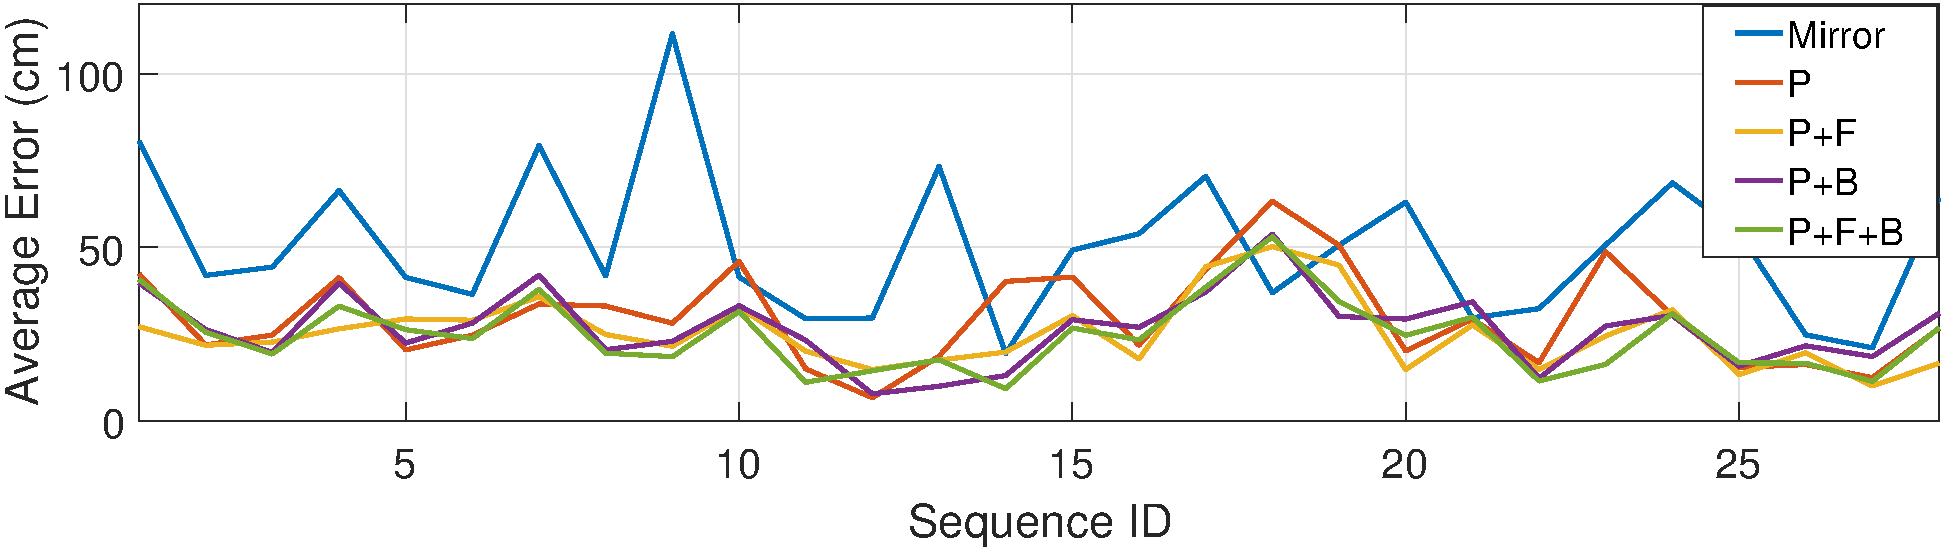
\includegraphics[width=\linewidth]{ssp_fig/cvpr19_predForm}\\
%	\includegraphics[width=\linewidth]{ssp_fig/cvpr19_predBody}
%	\caption{Average error of social formation prediction (top) and body gesture prediction (bottom). $y$-axis for the position errors in centimeters, and $x$-axis is sequence IDs.} %``Mirror" represents the baseline method, and P, F, and B denote Position, Face orientation, and Body orientation, as the input for the prediction.} 
%	\label{fig:predForm_errors}
%\end{figure}



% %Body only
% total_avg_posErr: 29.8286890398, std 13.3812589645
% total_avg_bodyOriErr: 0.263378293988, std 0.124290071428
% total_avg_faceOriErr: 0.327747834313, std 0.129691809416

% %Body + face
% total_avg_posErr: 25.2330815723, std 9.74251270294
% total_avg_bodyOriErr: 0.228412316901, std 0.0890485420823
% total_avg_faceOriErr: 0.303724261948, std 0.116639345884

% %Body + bodyOri
% total_avg_posErr: 26.57, std 10.24
% total_avg_bodyOriErr: 0.22, std 0.08
% total_avg_faceOriErr: 0.30, std 0.10

%While lower error may mean a better result, we may still see whether the prediction behave as human. 
% {\color{red} What happen when the turns are changing }

% {\color{red} Failure cases?}

% Position only, and orientation. 

% W/Wo speaking

% W/Wo body signal

% PCK curves

% Baseline: Trianglular estimation
% Orientation: See always the buyer.

% \begin{figure}
% 	\centering
% 	\includegraphics[width=\linewidth]{plot/cvpr19_predBody}
% 	\caption{Average error of body prediction. $y$-axis for the errors in centimeter, and $x$-axis for the sequences.} 
% 	\label{fig:predBody_errors}
% \end{figure}

\begin{figure*}
	\centering       
	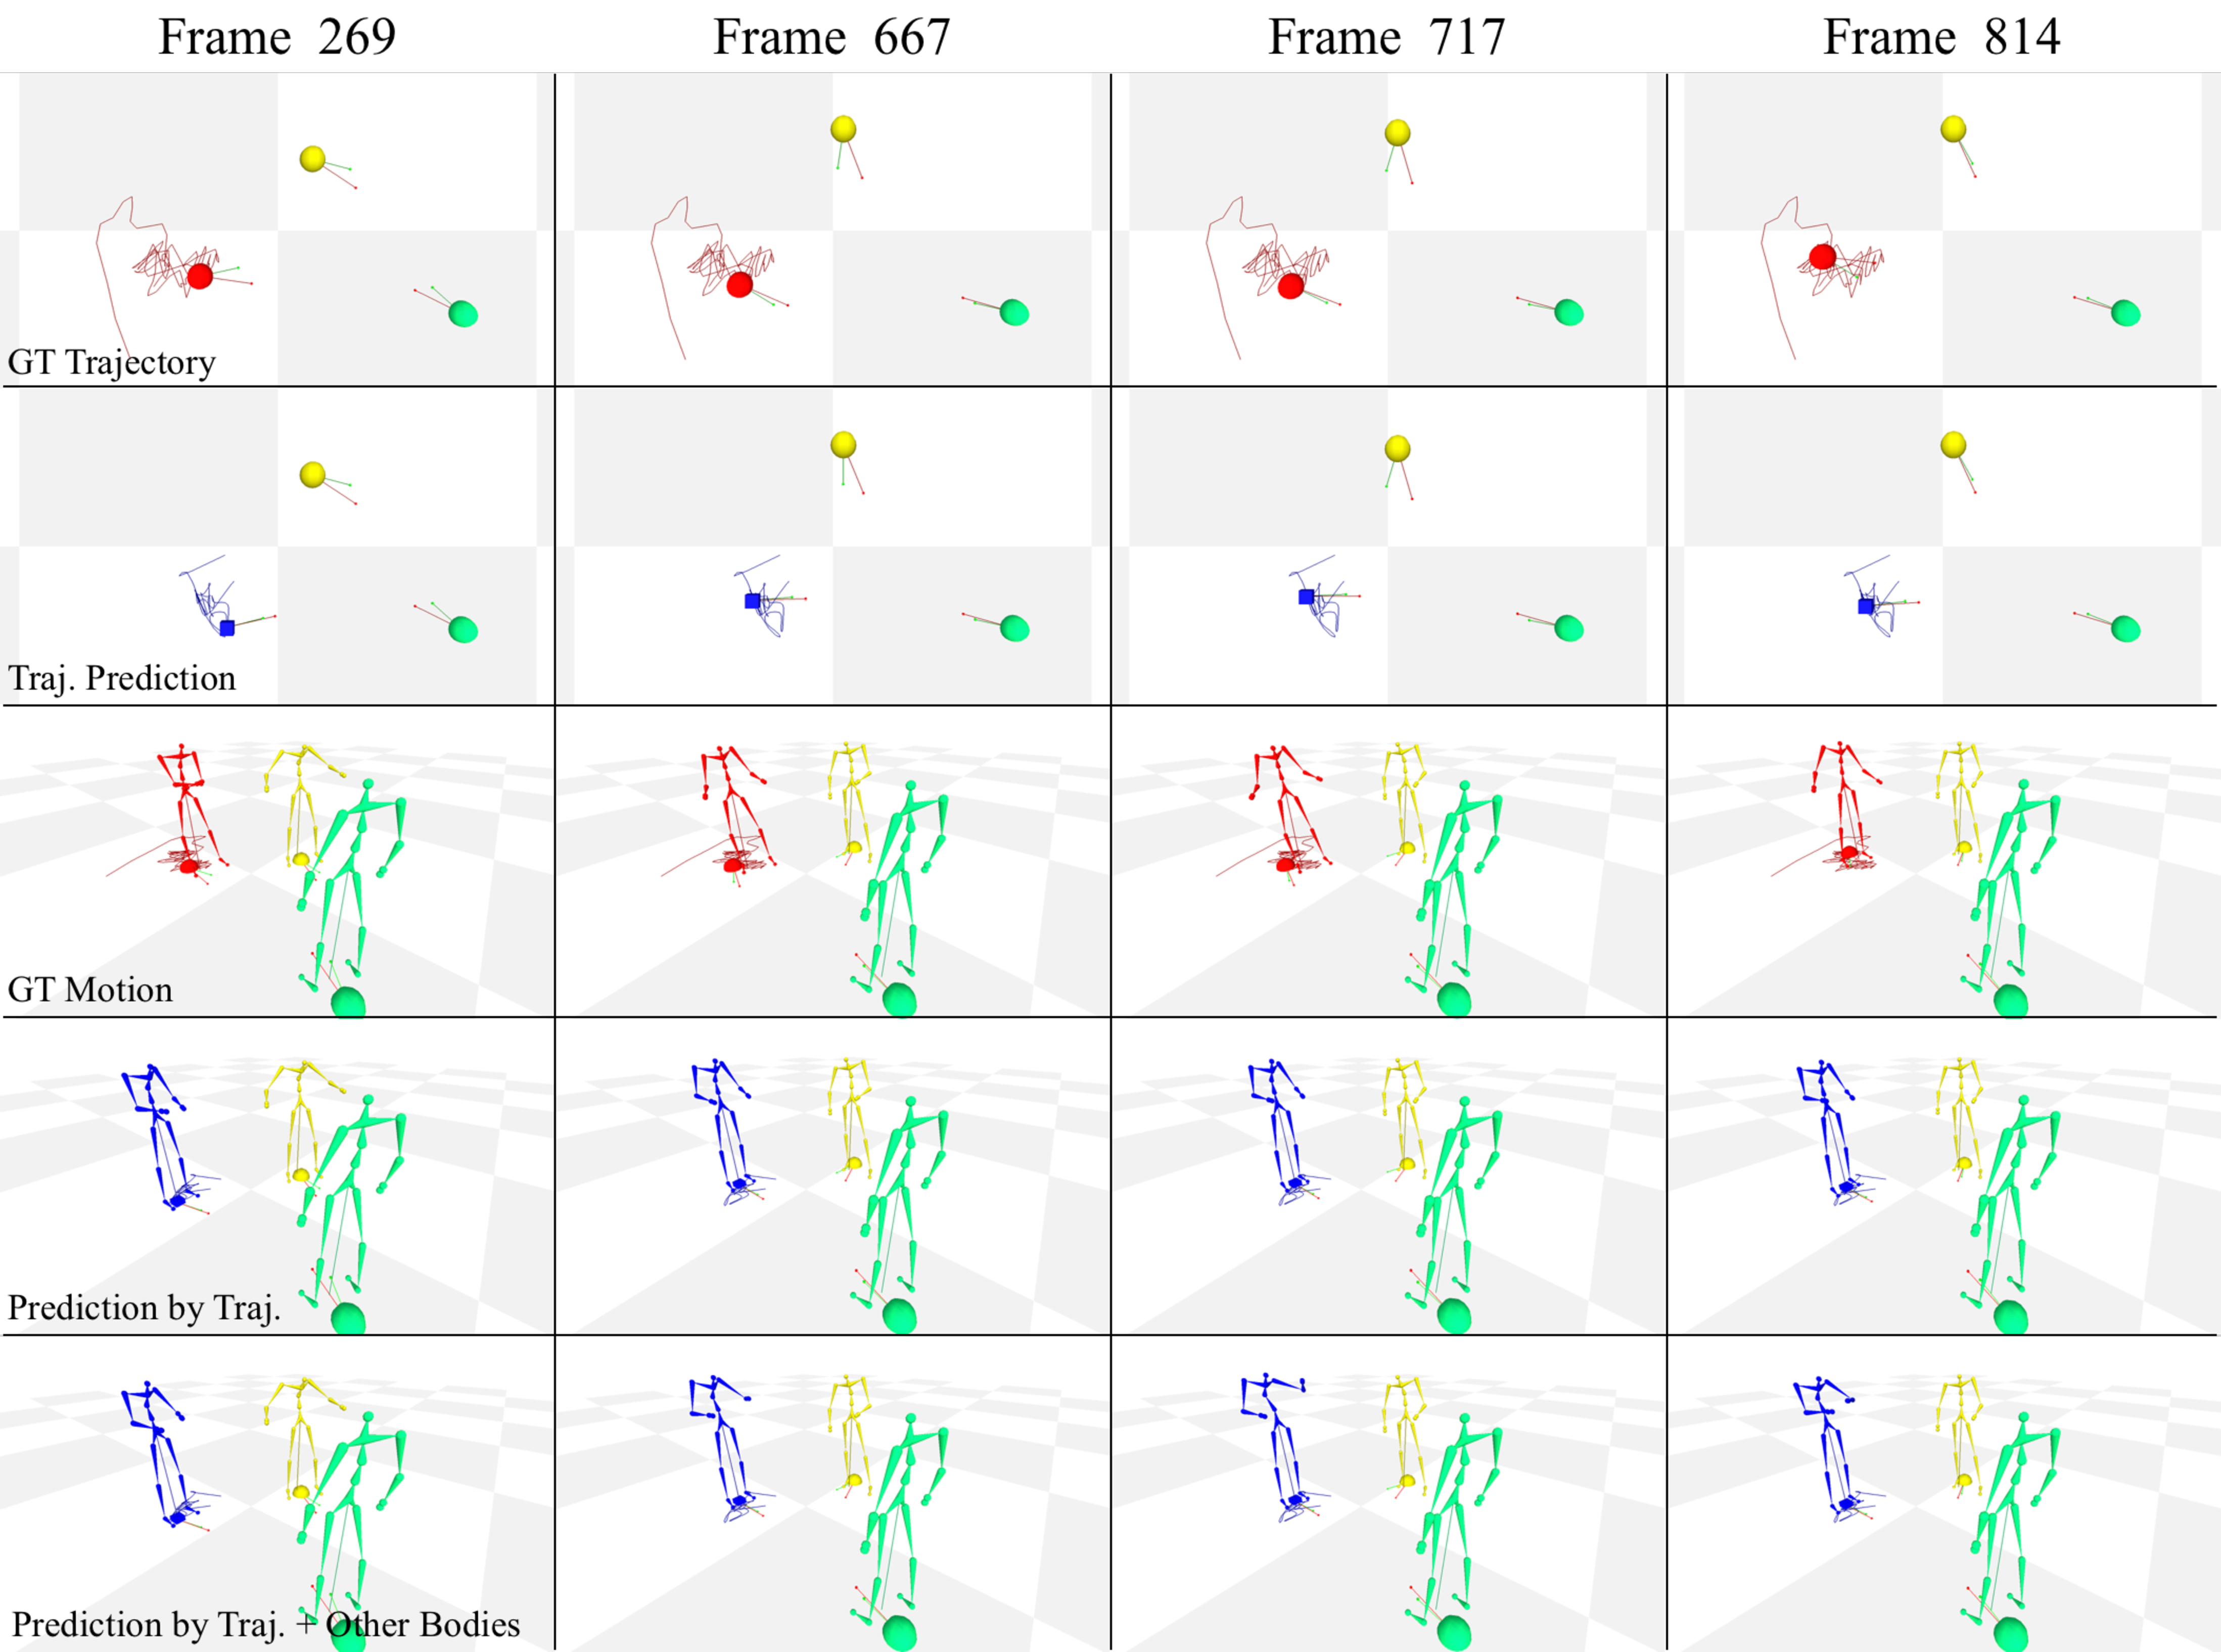
\includegraphics[width=\linewidth]{ssp_fig/qual_170221_b2_group4}
	%	\subfigure[TrajCompares]{\label{Fig:asso_traj}\includegraphics[width=0.5\textwidth]{img/trajCompare}}   
	\caption{An example result of \textit{Social Signal Prediction}. Each column shows scenes at a particular frame. The social signals drawn in green or yellow color are used as the inputs to our method, and blue signals are our social signal prediction results. The signals drawn in red are the ground truth. (First row) The ground truth social formations are shown from a top view, where the target person is shown as red spheres along with trajectories (red curves), face orientation (green arrows pointing from the spheres), and body orientations (red arrows from the spheres). (Second Row) The predicted locations (blue cubes), trajectories (blue curves), face orientations (green arrows), and body orientations (red arrows) are shown. (Third row) The ground-truth 3D body poses of the target person are shown. (Fourth row) We predict the 3D motion from the estimated 2D trajectory of the target person. (Fifth row) We use the body motion of other subjects to predict the upper body motion of the target person, which are combined to the leg body motions estimated from the trajectories.} 
	\label{fig:qualitative}
\end{figure*}

\begin{table}[t]
	\centering
%	\footnotesize
	%\caption{Social Body Gesture Prediction Errors}
	\begin{tabular}{c| c| c}
		
		\hline
		%Types & Avg. dist. (cm) & Std.(cm) & Min dist. (cm)  & Max dist. (cm)\\
		Types & Avg. Joint Errors (cm) & Std.\\
		\hline
		%Mirroring buyer & 11.60 &2.70\\
		%\hline
%		Mirroring input seller & 10.86 &2.49\\
%		\hline
		Mean Pose \underline {\textbf{7.83}} & 2.33\\
		\hline
		Traj2Body & 8.31 & 2.26\\
		\hline
		% 		body2Body & 8.19 (2.01)\\
		Body2Body & 8.72 & 2.00\\
		\hline
		% 		body2Body & 8.19 (2.01)\\
		Traj2Body (lower body) + Body2Body (upper body) & 8.61  & 1.84\\
		\hline
	\end{tabular}
	\caption{Social Body Gesture Prediction Errors (cm). Body orientation and face orientation are computed between estimated and GT unit vectors (need to be fixed) \label{table:predBody_errors}}
\end{table}



\begin{table}[t]
	\centering
	%	\footnotesize
	\begin{tabular}{l| l}
		\hline
		%Types & Avg. dist. (cm) & Std.(cm) & Min dist. (cm)  & Max dist. (cm)\\
		Input Signal & Accuracy\\
		\hline
		\hline
		Ground-truth Own Body & 79.94 \% \\       %new
				\hline
		Ground-truth Other Seller's Body & 75.28 \% \\       %new
		\hline
		\hline
		Mean Pose & 51.03\% \\       %new
				\hline
		Traj2Body & 51.42\% \\       %new
				\hline
		Body2Body & 52.97\% \\       %new
				\hline
		Body2Body+Traj2Body & 52.78\% \\       %new
				\hline
		Face2Body & \underline {\textbf{67.68}}\% \\       %new
				\hline
		Face2Body+Traj2Body & 66.60\% \\       %new
		\hline
	\end{tabular}
	\caption{We evaluate the speaking status of predicted models to quantitatively measure the quality of them. This table shows speaking status prediction accuracies, where the speaking status is predicted from the synthesized body motions from the specified sources.\label{table:pred_body_error_speaking}}
\end{table}



\subsection{Body Gestures Prediction}
As described in Section~\ref{section:pred_body}, we predict body motion of the target person by three different sources, which we refer to as: traj2body, body2body, and face2body. In the ``traj2body" method, the body motion is directly regressed from the estimated social formation (location and orientation) of the target person. This method shows reasonable leg motions following the trajectory movements, but has minimum upper body motion. Examples are shown in the fourth row of Fig.~\ref{fig:qualitative}. In ``body2body" method, we predict the target person's body motion by using other subjects' body motion as input. This motion does not take into account the global formation cues, but shows more dynamic body motions by responding to other subjects' motion. We can combine both methods, by merging the formation and leg motion from the first method to the upper body motion from the second method. Examples are shown in the fifth row of Fig.~\ref{fig:qualitative}. In the ``face2body" method, we use other seller's face motion as a source to predict the body motion of the target person. Similarly, we can combine this output with the leg motion of ``traj2body" method. The prediction results show human-like social behaviors including location, body and face orientation, leg motion, and hand gestures. 

We first quantitatively evaluate the predicted body gesture using the common L2 distance. We consider a baseline method, ``Mean Pose", by computing the average posture of all training data and constantly use it as prediction output. As shown in Table~\ref{table:predBody_errors}, the L2 error of this baseline shows the best performance, although this motion is not realistic and not suitable for social situations.

For our new metric described in Section~\ref{section:evaluation}, we predict the speaking status from the predicted motions. We use our pre-trained speaking status classifier that takes own body signals as input, which shows about $76\%$ prediction accuracy in Table~\ref{table:speaking_class}. Then, we compute the speaking status accuracy using ground truth speaking status. The speaking is closely related to the turn-taking timing in the interaction, and this method penalizes if the predicted body motion does not follow the speaking timing of the ground truth data. As shown in Table~\ref{table:pred_body_error_speaking}, the baseline method using the mean pose only shows almost a chance level accuracy ($51.03\%$), showing mostly no speaking motions regardless the situations\footnote{The position and orientation part of the input values are still changing, which makes sometimes our classier produces speaking label as output.}. The prediction by ``body2body" method shows a better performance, but still poor in this metric. The prediction by `` face2body" method shows the best performance with a significant margin, since, presumably, the face cue of other subjects provides a strong clue to determine the speaking timing, as demonstrated in Table~\ref{table:speaking_class}. This experiment shows interesting correlations among position, orientation, body, and face signals among interacting groups. %As shown in this result, our social signal prediction method shows a reasonable performance in modeling the dynamics of social signals, and our evaluation method can be used to quantify the output.


%The final outputs predict more natural social behaviors than other baselines, satisfying most of the noticeable social rules in the scenes (distance, orientation, leg and root movement, and natural hand motions). Our results are best seen in the supplementary videos. However, the quantitative errors tend to be higher, as shown in Table~\ref{table:predBody_errors} and Figure~\ref{chapter:predBody_errors}. Notably, the average pose computed from the training set shows the best performance. This is because the error metric computing the 3D errors from the ground-truth cannot fully evaluate how natural the motion appears. %Given the similar social signal inputs, there are diverse possible suitable human motions, and a better evaluation method is required to consider this.%  the quality of social signal prediction.% and it should be related to a 

% {\color{red} Qualitative example where turn taking is captured?}

% \noindent \textbf{Direct Regression from Social Formations:}
% We can directly regress from the predicted 2D formation output.  

% PCK curves 
% Per joint


% \textbf{Regression from Richer Input:}
% We use other skeletons and input and see any improvement. 

% Compared to the direct regression. 
% {\color{red} Any semantic improvement which is not captured by numbers?}

% Any good way to evaluate realistic human motion???


% \subsection{Quantifying Social Signal Importance}



% \subsection{Correlation between Body, Face, and Hands}

% We use all body parts for communication where each part plays a role to send some specific signals. Unfortunately, these roles are also poorly understood. In this section, we investigate whether there exists patterns or strong correlations among parts. We study this by predicting a missing part given other body parts. 

% Body2face, face2body

% \subsection{Face and Hands signals}